\documentclass[a4paper, 11pt]{article}
\usepackage[polish]{babel}
\usepackage[T1]{fontenc}
\usepackage{hyperref}
\usepackage{array}
\usepackage{amssymb}
\usepackage[margin=1in]{geometry}
\hypersetup{
    colorlinks,
    citecolor=black,
    filecolor=black,
    linkcolor=black,
    urlcolor=black
}
\usepackage{graphicx}

\usepackage{tikz}
\usetikzlibrary{fit,arrows,matrix,positioning, calc, shapes.gates.logic.IEC, shapes.gates.logic.US}
\tikzstyle{branch}=[fill,shape=circle,minimum size=3pt,inner sep=0pt]


\title{%
	%\vspace{-3.5cm}
       \large Sprawozdanie Laboratorium Mikroelektronika \\
       \huge  Inwerter CMOS}

\author{Stanisław Fiedler 160250 L1}
\date{LAB 3 oraz 4, 5 listopada 2024}

\begin{document}

\maketitle
\tableofcontents

\section{Symulacja tranzystora NMOS}\label{sec:symulacja_tranzystora_nmos} % (fold)
W schemacie na rysunku 1 (z poprzednich zajęć) dokonać zmiany wartości szerokości kanału tranzystora
nMOS z W=10u na W=5u. Następnie dokonać ponownej symulacji układu. Zinterpretować uzyskane wyniki w
odniesieniu do wzorów opisujących zasadę działania tranzystora nMOS.

\begin{center}
	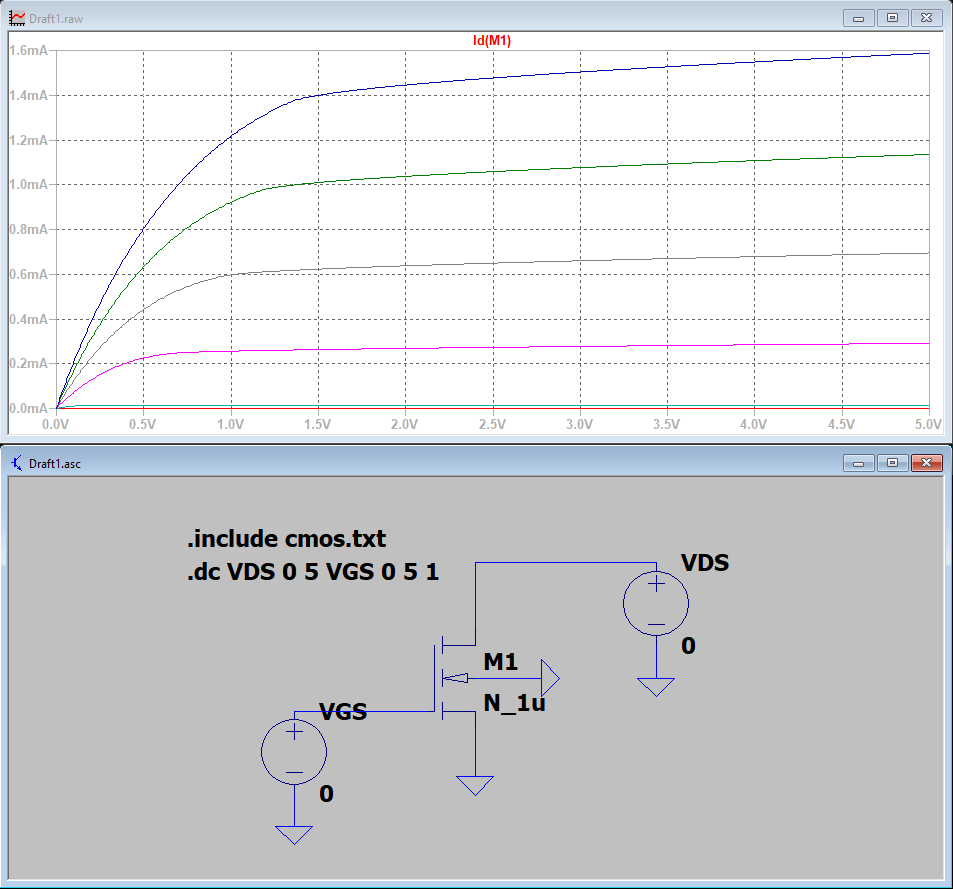
\includegraphics[scale=0.4]{mikro_lab3/Przechwytywanie.PNG}
\end{center}

\[
	I_D = \mu C_{OX} \frac{W}{L} \frac{\left( V_{GS} - V_{T} \right)^2}{2}
\]

Ze wzoru wynika że prąd płyn płynący przez tranzystor jest wprost proporcjonalny do szerokości kanału W. Zwężenie kanału o połowę zmniejszyło płynący prąd również o połowę.

% section Symulacja tranzystora NMOS (end)

\section{Symulacja inwertera CMOS}\label{sec:symulacja_inwertera_cmos} % (fold)
Dokonać symulacji obwodu z rysunku 2. W oknie wyników symulacyjnych, pod prawym przyciskiem
wybrać Add plot pane. Napięcie wejściowe i wyjściowe wyświetlić w niezależnych sekcjach (‘plot pane’). Analizując
wyniki uzyskanej symulacji dokonaj interpretacji zasady działania inwertera CMOS.

\begin{center}
	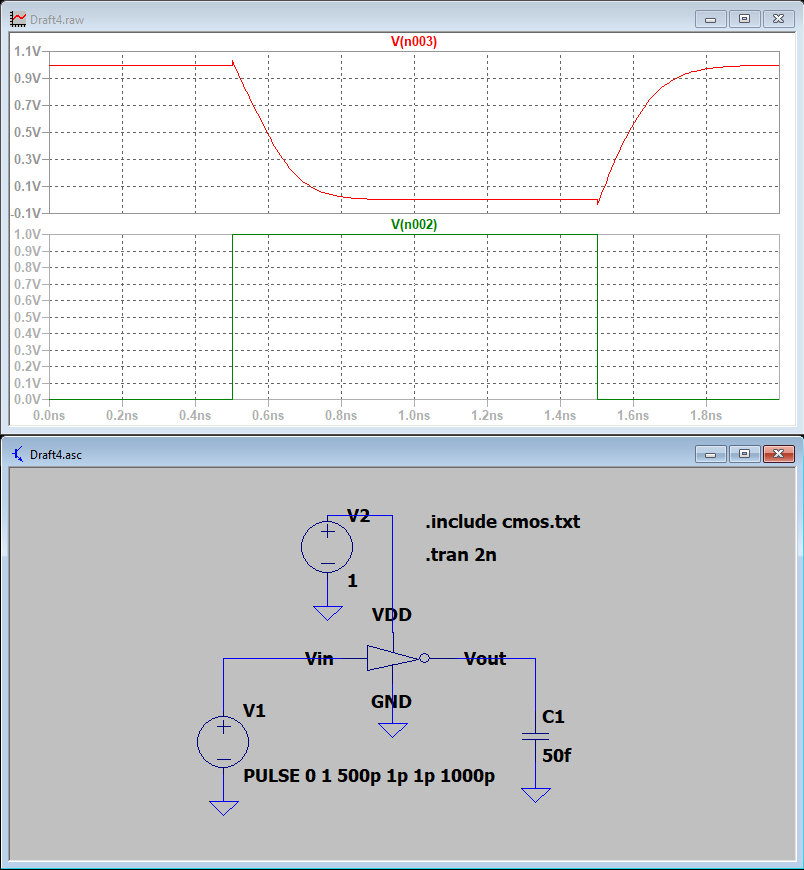
\includegraphics[scale=0.4]{mikro_lab3/Przechwytywanie2.PNG}
\end{center}

Inwerter CMOS jest implementacją bramki logicznej not.
Kiedy na $V_{in}$ jest 0V na wyjściu $V_{out}$ jest napięcie $V_{DD}$.
Kiedy na $V_{in}$ jest napięcie $V_{DD}$ na wyjściu $V_{out}$ jest 0V.

% section Symulacja inwertera CMOS (end)
\section{Dlaczego długości oraz szerokości kanałów dla tranzystorów pMOS i nMOS nie są jednakowe?}\label{sec:WL} % (fold)

Aby tranzystory pMOS miał charakterystyki podobne do tranzystora nMOS rozmiar jego kanał musi być większy. Jest to spowodowane mniejszą ruchliwością dziur elektronowych w porównaniu z elektronami.

% section WL  (end)

\section{Parametry inwertera}\label{sec:parametry_inwerter} % (fold)

Dla symulacji z rysunku 2 wyznaczyć parametry rise time, fall time, edge rate, high-to-low propagation
delay, low-to-high propagation delay, propagation delay, contamination delay.

\begin{description}
	\item[Rise time:] $198 ps$ \hfill
	      \begin{center}
		      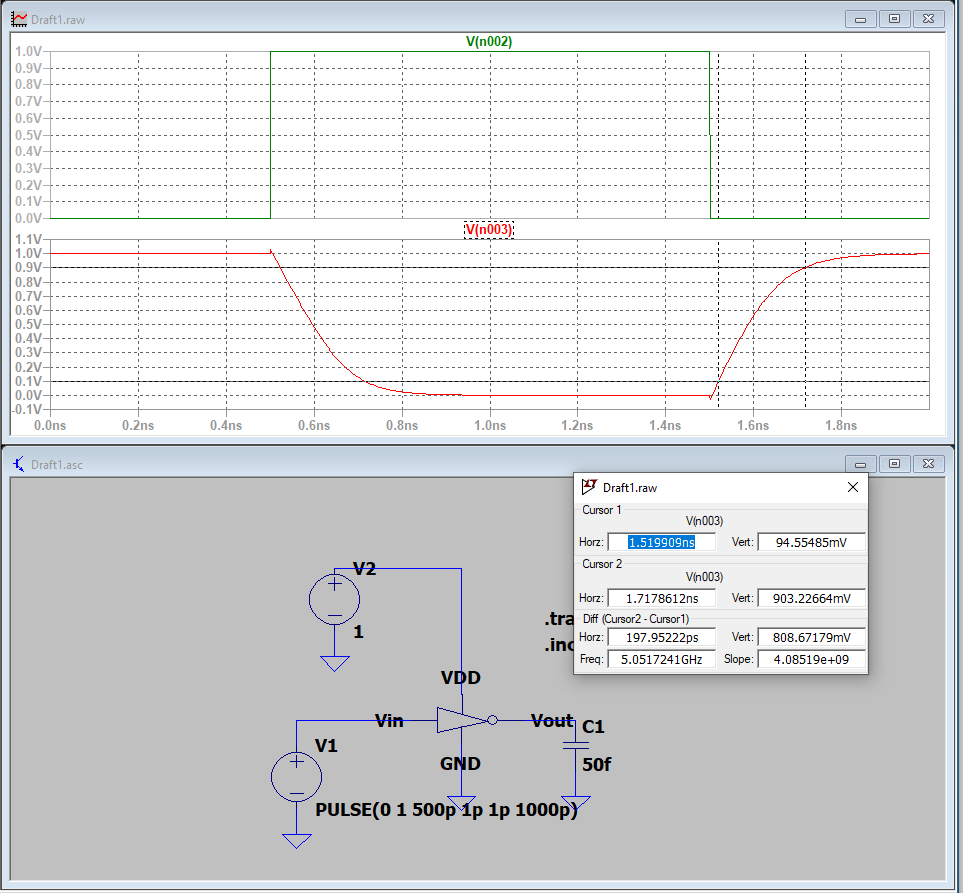
\includegraphics[scale=0.38]{mikro_lab3/rise_time.PNG}
	      \end{center}
	      \pagebreak
	\item[Fall time:] $200 ps$ \hfill
	      \begin{center}
		      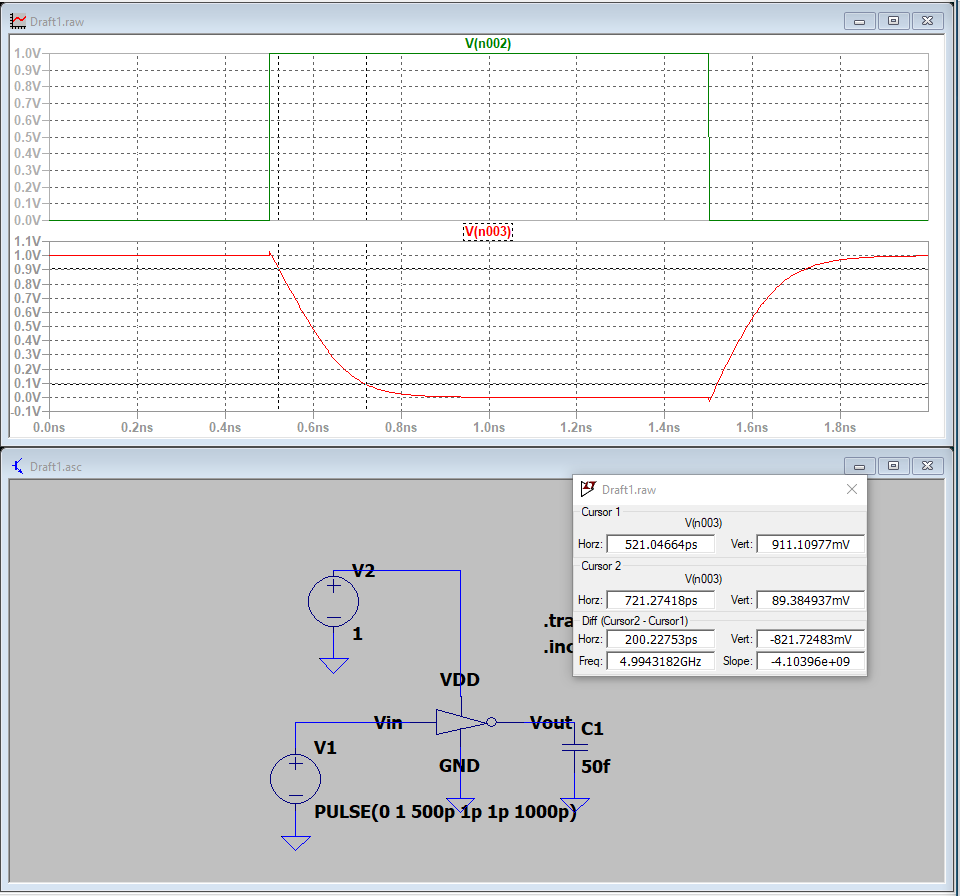
\includegraphics[scale=0.38]{mikro_lab3/fall_time.PNG}
	      \end{center}
	\item[Edge rate:] $\frac{198ps + 200ps}{2} = 199ps$
	\item[High-to-low propagation delay:] $98ps$ \hfill
	      \begin{center}
		      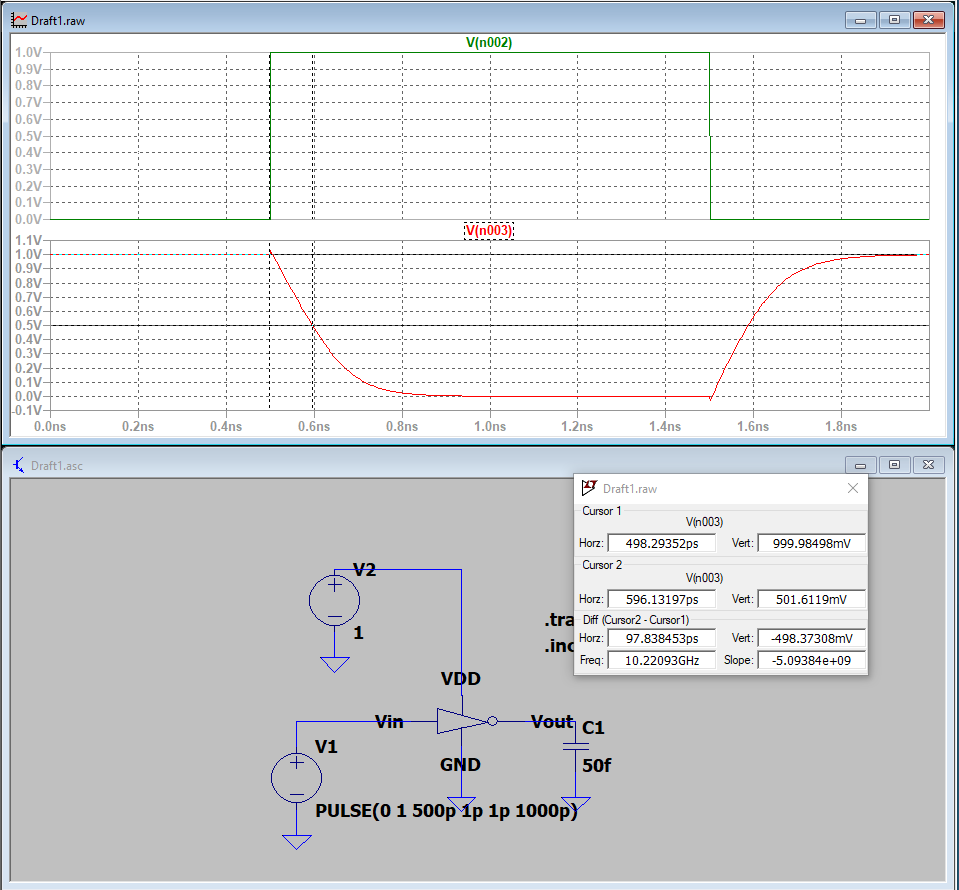
\includegraphics[scale=0.38]{mikro_lab3/high_to_low.PNG}
	      \end{center}
	      \pagebreak
	\item[Low-to-high propagation delay:] $89ps$ \hfill
	      \begin{center}
		      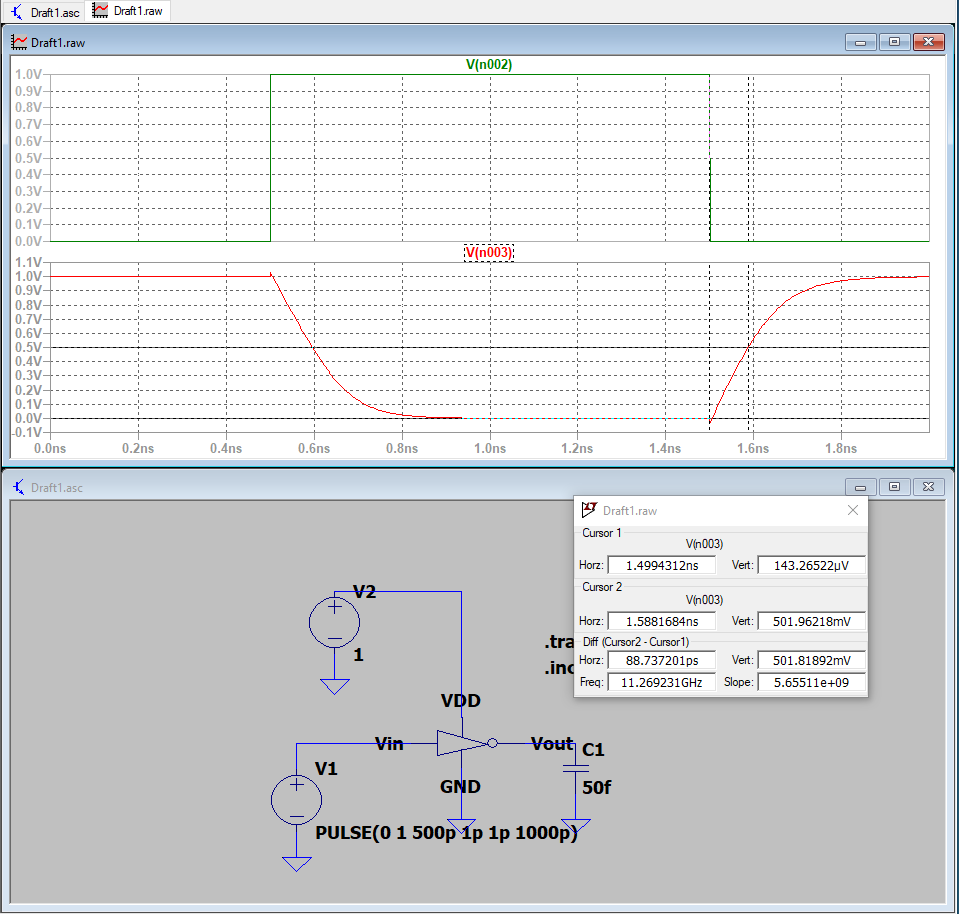
\includegraphics[scale=0.38]{mikro_lab3/low_to_high.PNG}
	      \end{center}
	\item[Propagation delay:] $\frac{98ps + 89ps}{2} = 93,5ps $
	\item[Contamination delay:] $ min\{98ps, 89ps\} = 89ps $
\end{description}

% section Parametry 1 inwerter (end)

\section{Parametry 4 połączonych szeregowo inwerterów}\label{sec: parametry_szeregowo} % (fold)

Opierając się na przykładzie z rysunku 2 zaprojektować układ złożony z połączonych szeregowo 4 bramek
logicznych not (inwerterów). Ostatni inwerter obciążyć pojemnościowo. Dla zaprojektowanego układu dokonać symulacji
oraz wyznaczyć parametry z poprzedniego punktu mierzone między portem wyjściowym na pierwszej bramce, a wyjściem
każdej kolejnej bramki not.

\begin{center}
	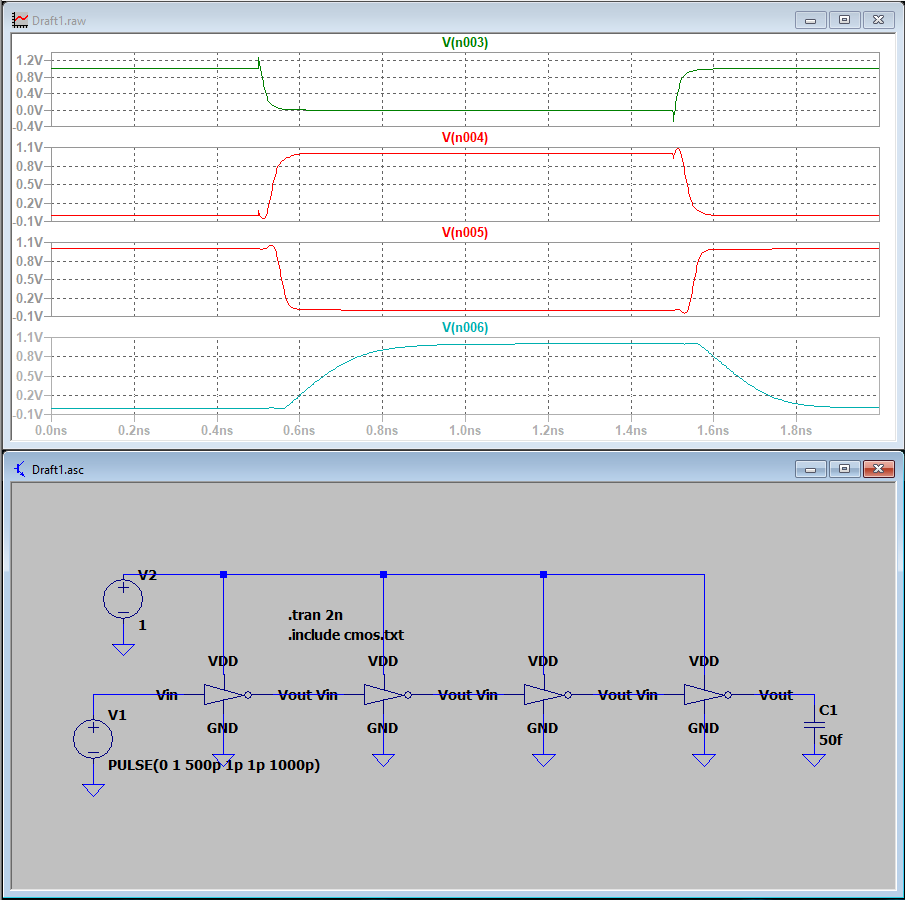
\includegraphics[scale=0.35]{mikro_lab3/symulacja4.PNG}
\end{center}

\subsection{Pierwszy inwerter}
\begin{description}
	\item[Rise time:] $37 ps$ \hfill
	      \begin{center}
		      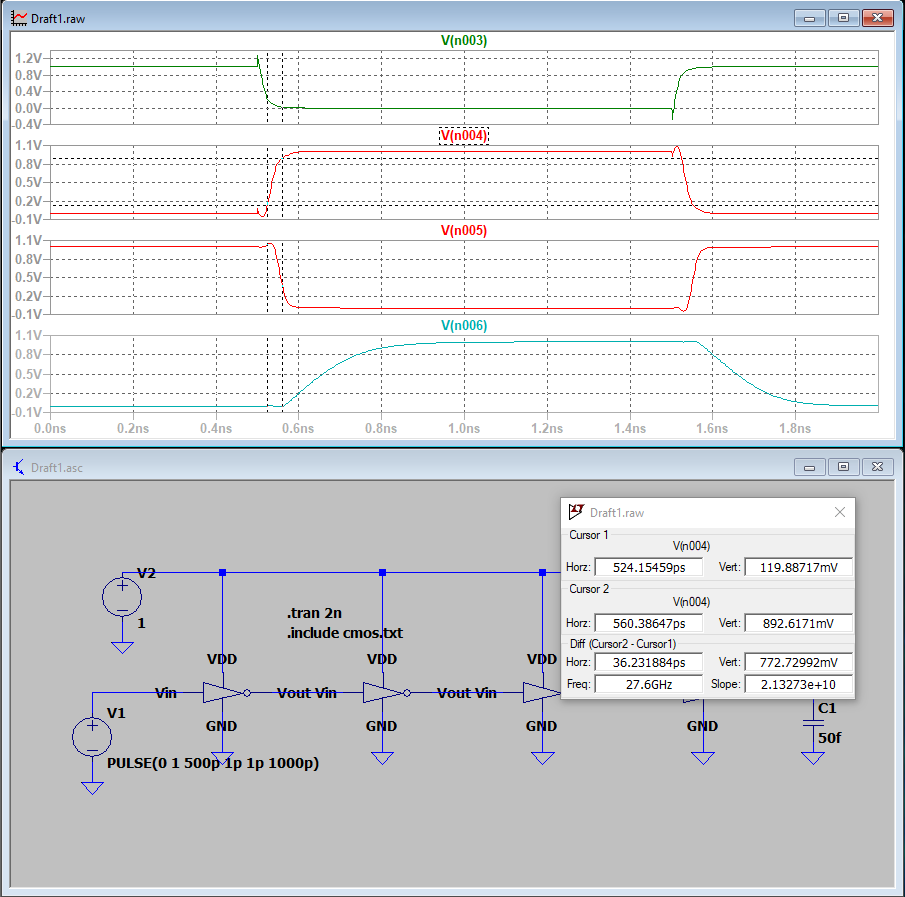
\includegraphics[scale=0.38]{mikro_lab3/rise_time1.PNG}
	      \end{center}
	\item[Fall time:] $33 ps$ \hfill
	      \begin{center}
		      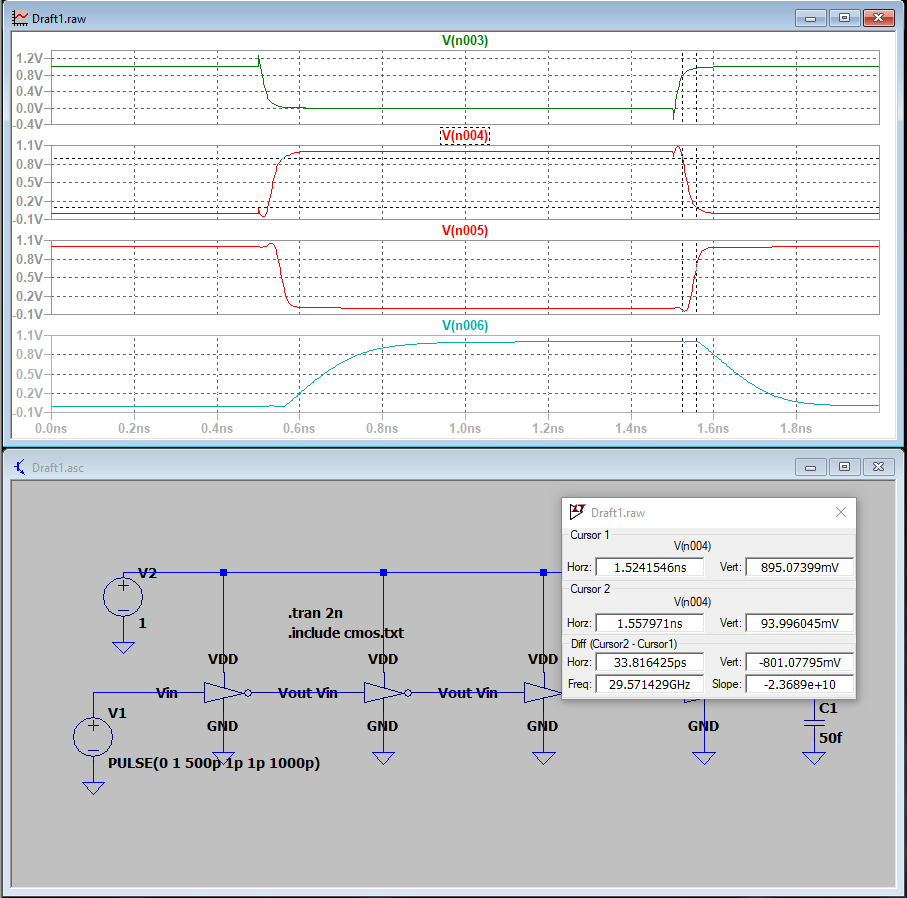
\includegraphics[scale=0.38]{mikro_lab3/fall_time1.PNG}
	      \end{center}
	\item[Edge rate:] $\frac{37ps + 33ps}{2} = 35ps$
	      \pagebreak
	\item[High-to-low propagation delay:] $22ps$ \hfill
	      \begin{center}
		      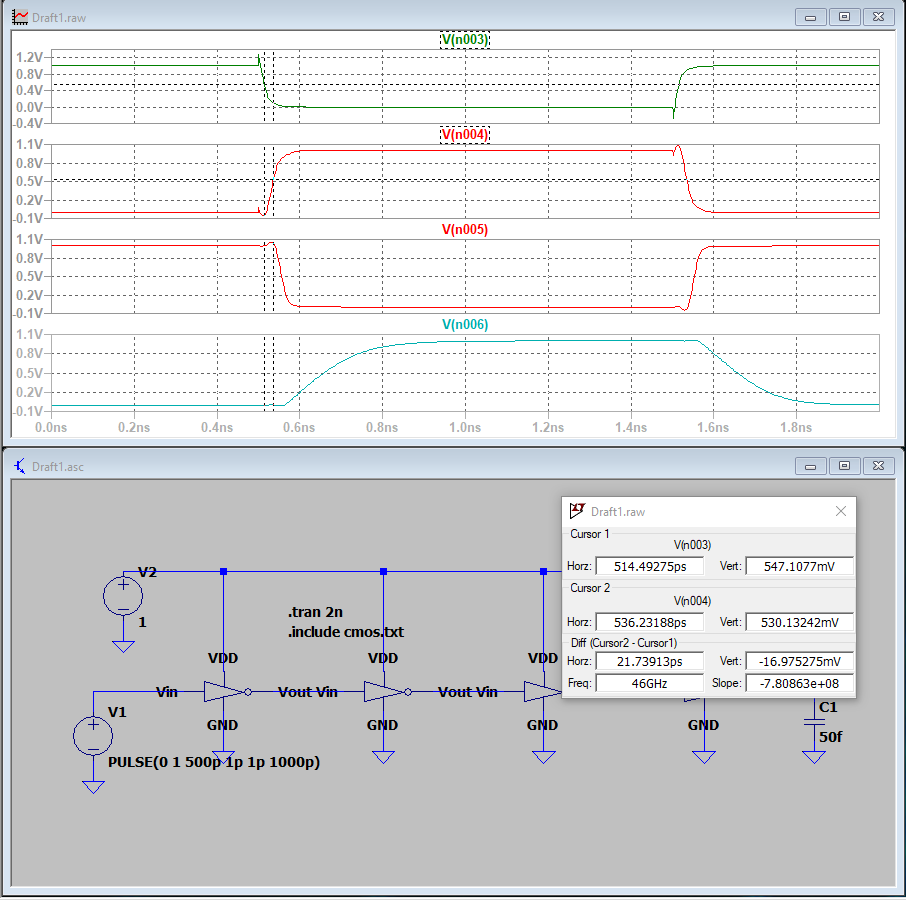
\includegraphics[scale=0.38]{mikro_lab3/high_to_low1.PNG}
	      \end{center}
	\item[Low-to-high propagation delay:] $19ps$ \hfill
	      \begin{center}
		      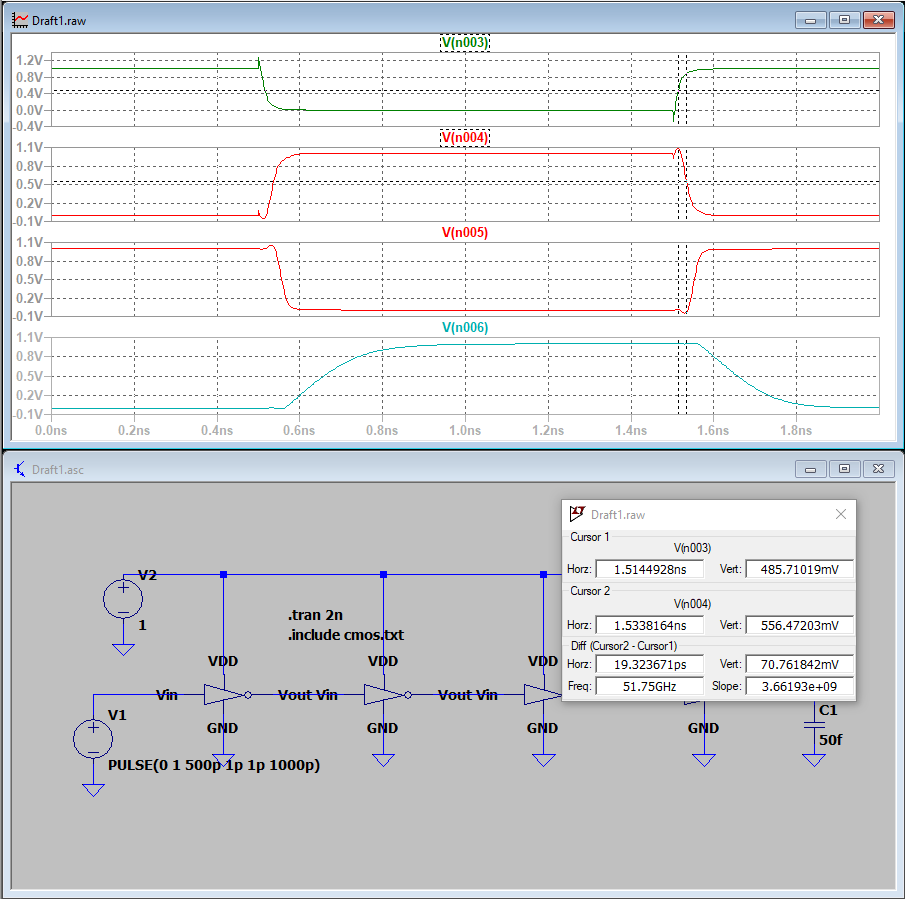
\includegraphics[scale=0.38]{mikro_lab3/low_to_high1.PNG}
	      \end{center}
	\item[Propagation delay:] $\frac{22ps + 19ps}{2} = 20,5ps $
	\item[Contamination delay:] $ min\{22ps, 19ps\} = 19ps $
\end{description}
% subsection inv1 (end)

\pagebreak
\subsection{Drugi inwerter}
\begin{description}
	\item[Rise time:] $29 ps$ \hfill
	      \begin{center}
		      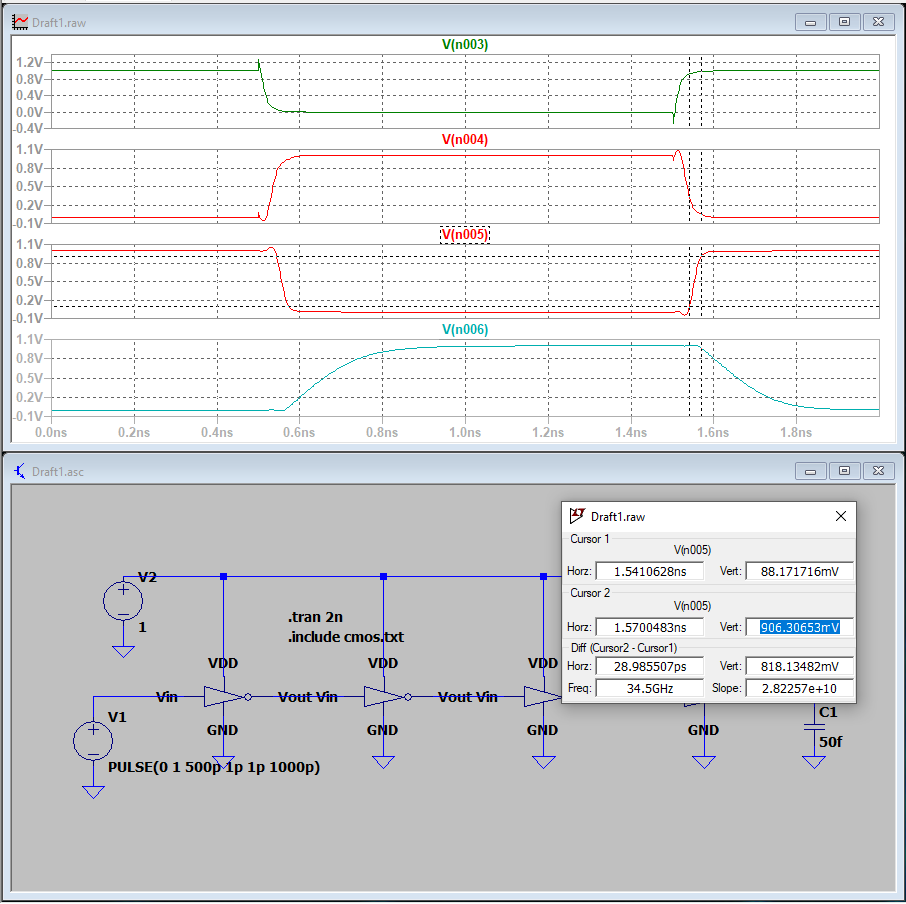
\includegraphics[scale=0.38]{mikro_lab3/rise_time2.PNG}
	      \end{center}
	\item[Fall time:] $31 ps$ \hfill
	      \begin{center}
		      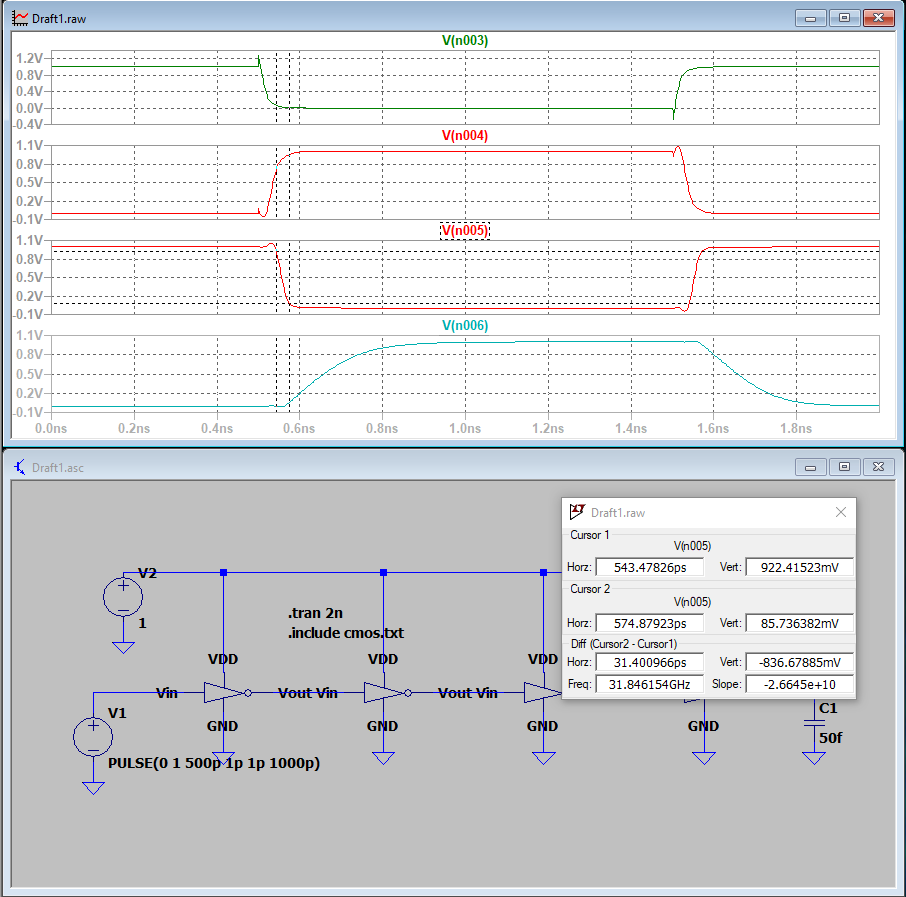
\includegraphics[scale=0.38]{mikro_lab3/fall_time2.PNG}
	      \end{center}
	\item[Edge rate:] $\frac{29ps + 31ps}{2} = 30ps$
	      \pagebreak
	\item[High-to-low propagation delay:] $41ps$ \hfill
	      \begin{center}
		      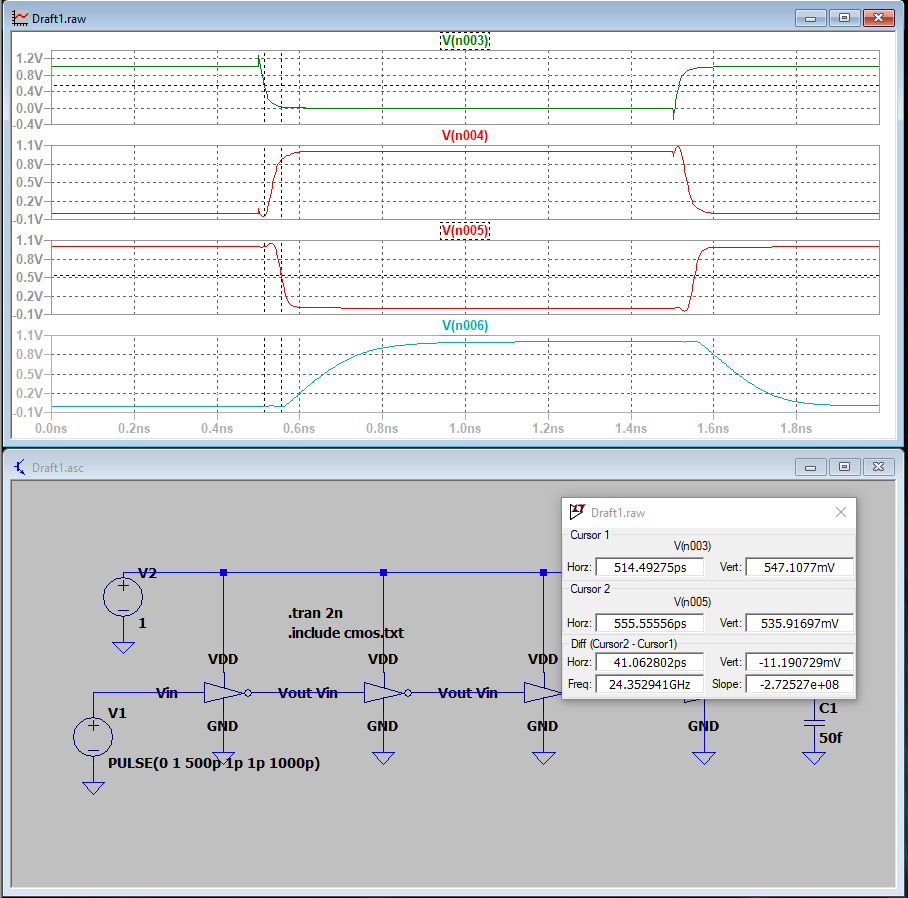
\includegraphics[scale=0.38]{mikro_lab3/low_to_high2.PNG}
	      \end{center}
	\item[Low-to-high propagation delay:] $39ps$ \hfill
	      \begin{center}
		      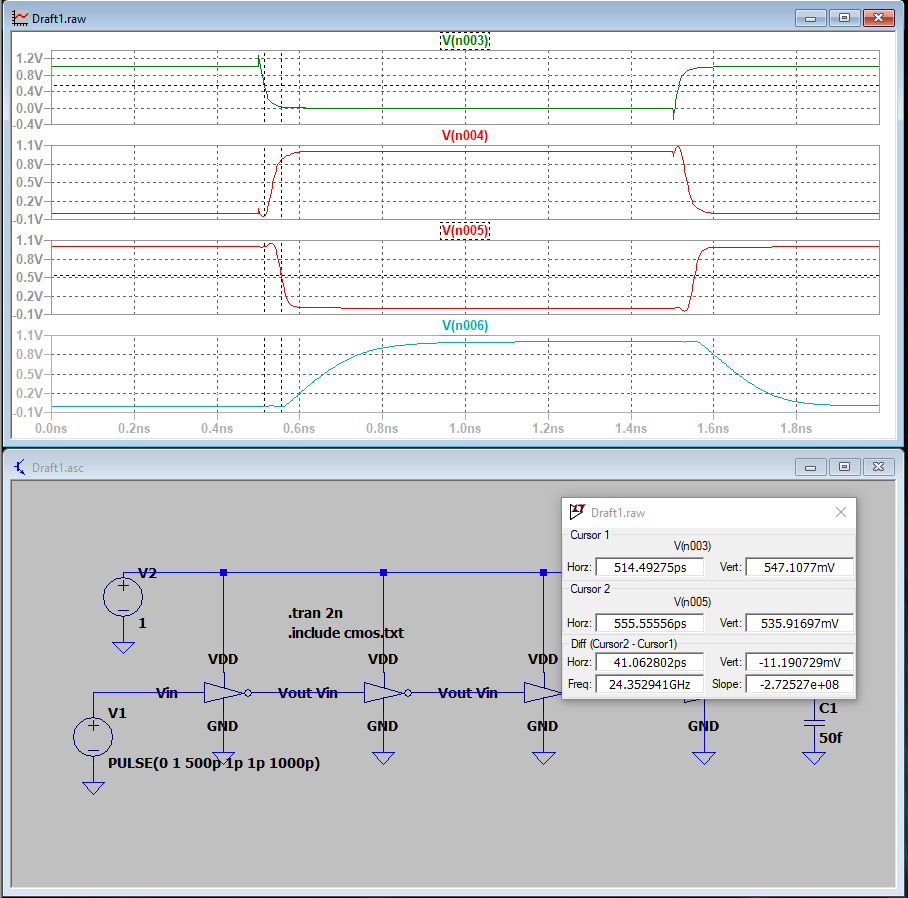
\includegraphics[scale=0.38]{mikro_lab3/low_to_high2.PNG}
	      \end{center}
	\item[Propagation delay:] $\frac{39ps + 41ps}{2} = 40ps $
	\item[Contamination delay:] $ min\{39ps, 41ps\} = 39ps $
\end{description}
% subsection inv2 (end)

\pagebreak
\subsection{Trzeci inwerter}
\begin{description}
	\item[Rise time:] $217 ps$ \hfill
	      \begin{center}
		      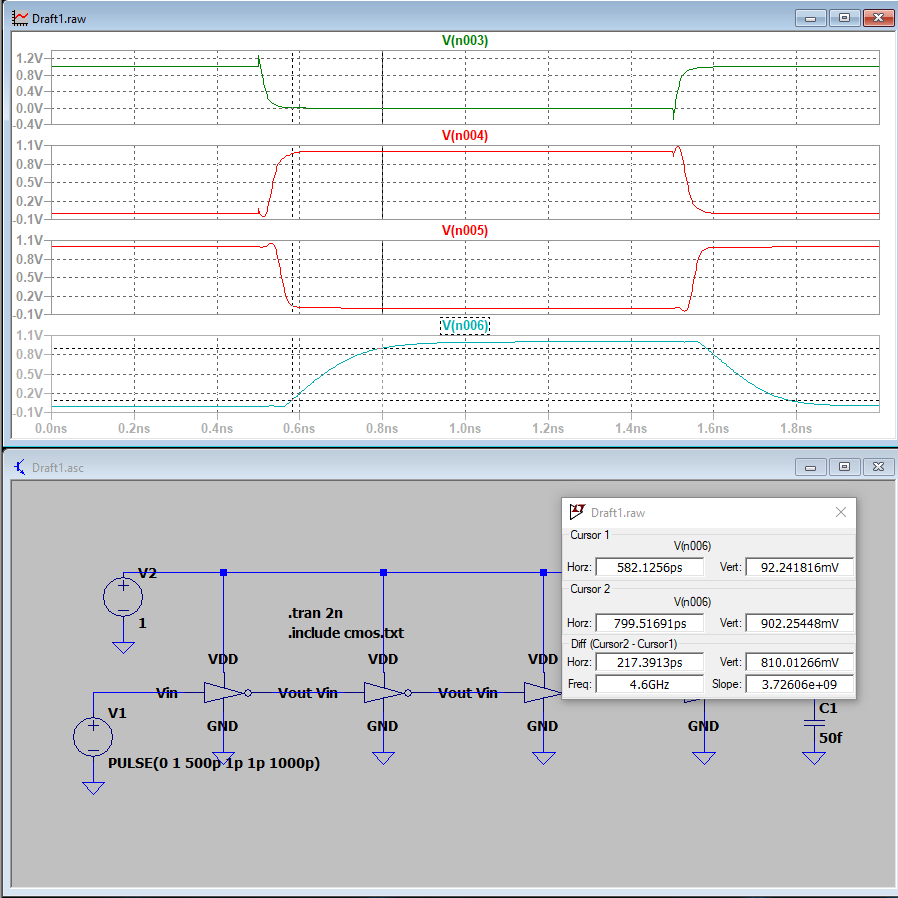
\includegraphics[scale=0.38]{mikro_lab3/rise_time3.PNG}
	      \end{center}
	\item[Fall time:] $193 ps$ \hfill
	      \begin{center}
		      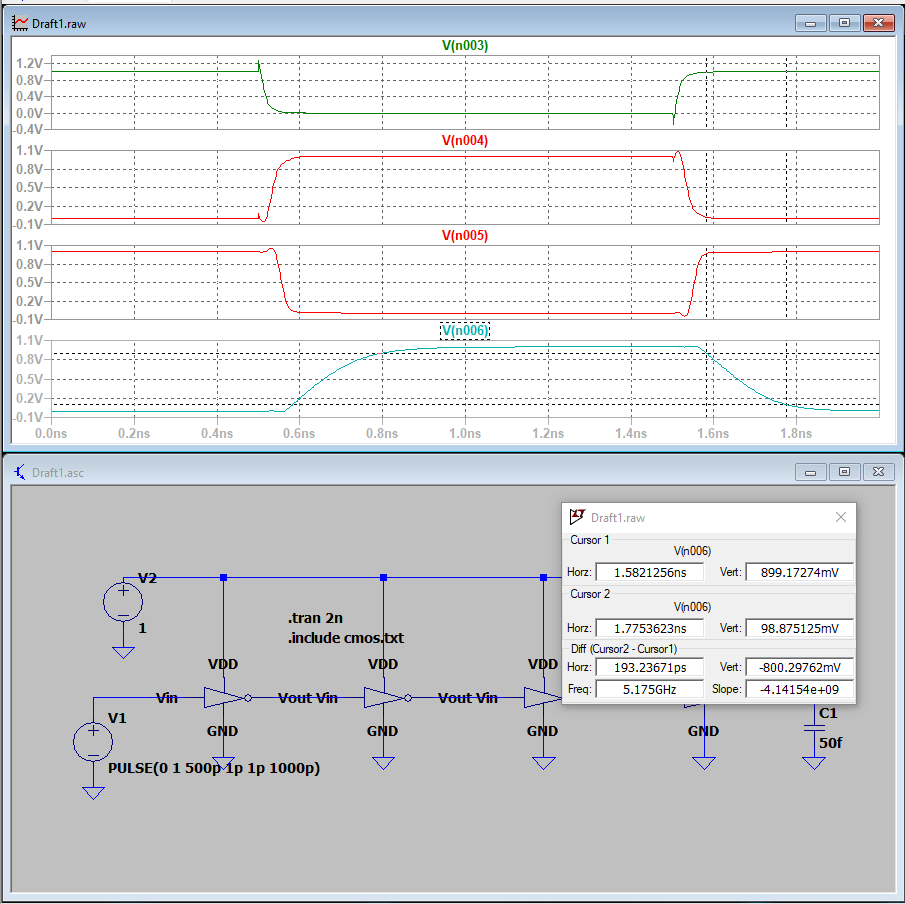
\includegraphics[scale=0.38]{mikro_lab3/fall_time3.PNG}
	      \end{center}
	\item[Edge rate:] $\frac{217ps + 193ps}{2} = 205ps$
	      \pagebreak
	\item[High-to-low propagation delay:] $140ps$ \hfill
	      \begin{center}
		      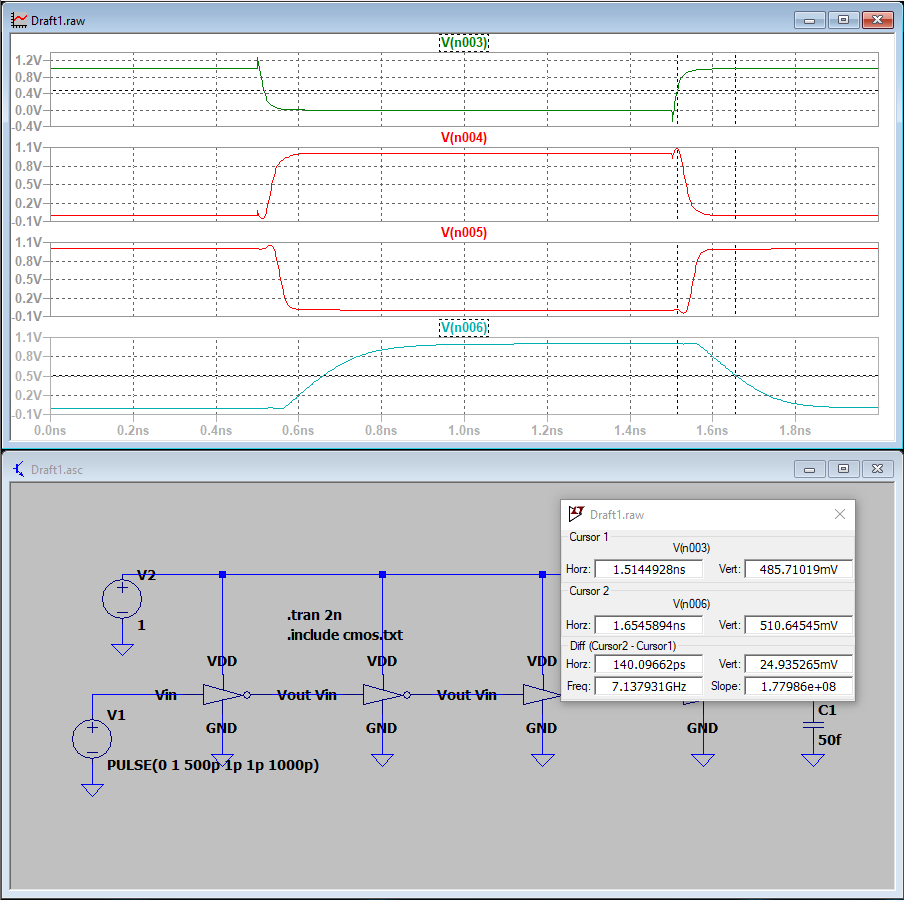
\includegraphics[scale=0.38]{mikro_lab3/high_to_low3.PNG}
	      \end{center}
	\item[Low-to-high propagation delay:] $140ps$ \hfill
	      \begin{center}
		      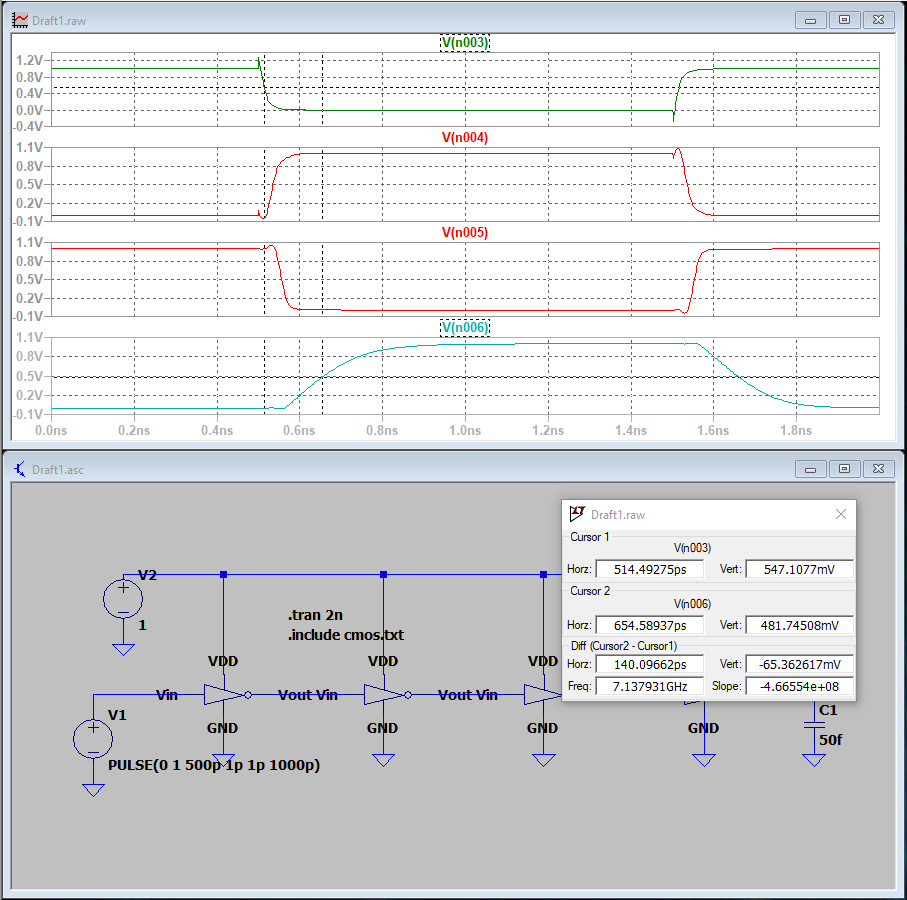
\includegraphics[scale=0.38]{mikro_lab3/low_to_high3.PNG}
	      \end{center}
	\item[Propagation delay:] $\frac{140ps + 140ps}{2} = 140ps $
	\item[Contamination delay:] $ min\{140ps, 140ps\} = 140ps $
\end{description}
% subsection inv3 (end)

\pagebreak

\section{Charakterystyka przejściowa symulacja}\label{sec:charakterystypa przejsciuowa} % (fold)
Na wyniku symulacyjnym oznacz obszary w których: M1-on, M2-off, M1-off, M2-on.

\begin{center}
	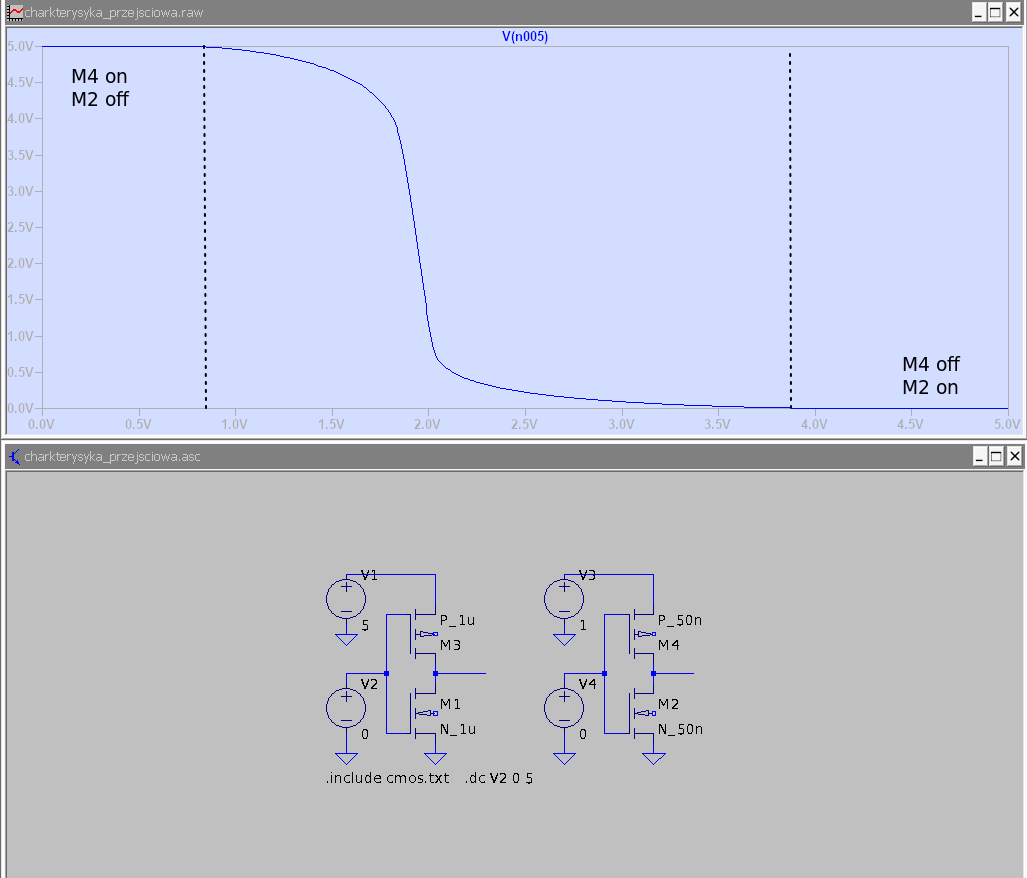
\includegraphics[scale=0.3]{images/sym_rysA.png}
	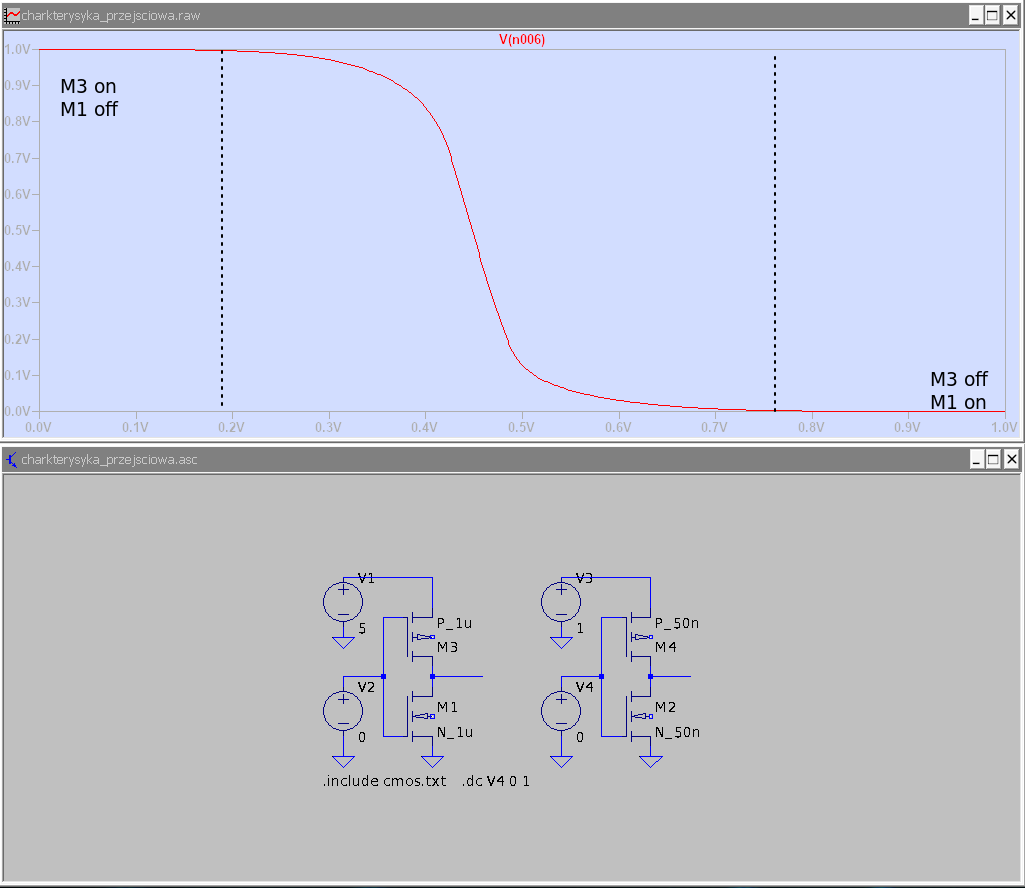
\includegraphics[scale=0.3]{images/sym_rysB.png}
\end{center}

% section  (end)

\section{Wyjaśnij co oznaczają oznaczenia VIL, VIH, VIH, VOH}\label{sec:oznaczenia} % (fold)

\begin{description}
	\item[$V_{IL}$] granica napięcia na wejściu interpretowanego jako niskie.
	\item[$V_{IH}$] granica napięcia na wejściu interpretowanego jako wysokie.
	\item[$V_{OL}$] napięcie na wyjściu w stanie niskim.
	\item[$V_{OH}$] napięcie na wyjściu w stanie wysokim.
\end{description}

% section  (end)

\section{Symulacja największy pobór prądu}\label{sec:poborpradu} % (fold)
Przedstaw wynik symulacyjny, obrazujący obszar, w którym następuje największy pobór prądu.
% section  (end)

\begin{center}
	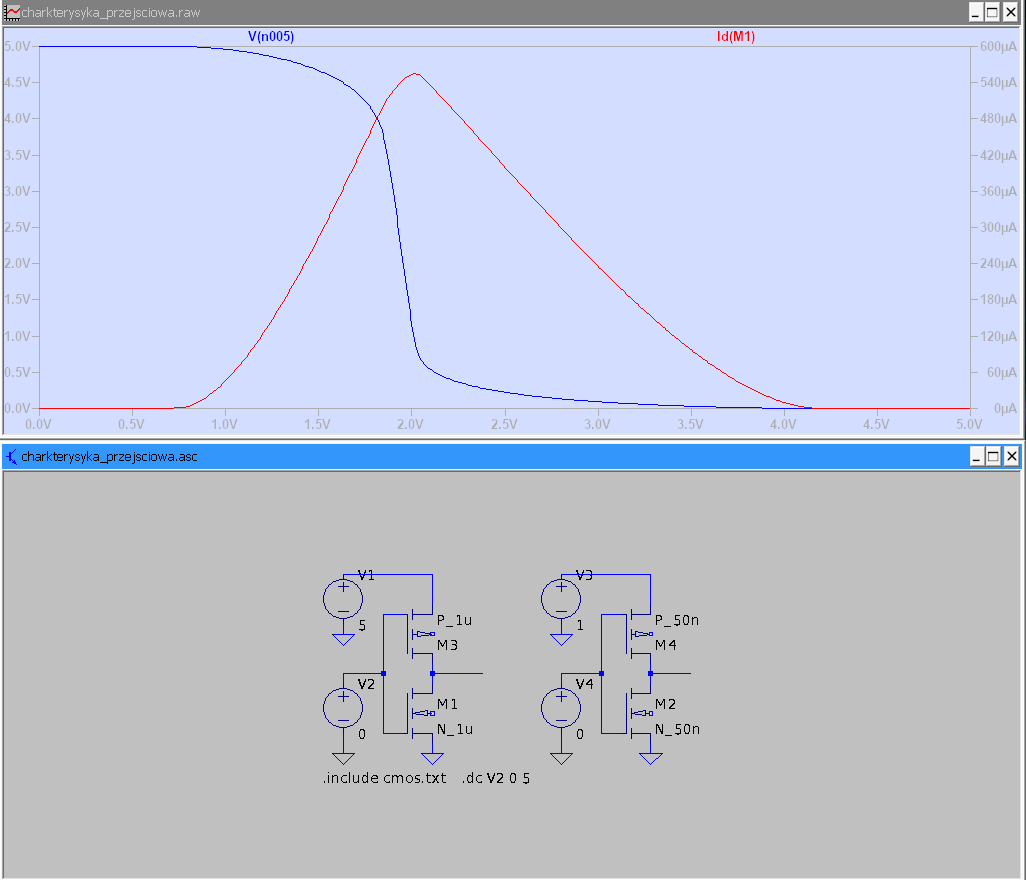
\includegraphics[scale=0.4]{images/pobor_pradu.png}
\end{center}

\section{Inverter Switching Point}\label{sec:nverter_switching_point} % (fold)
Wyznacz ‘Inverter Switching Point’ – napięcie VSP, w którym napięcie wejściowe jest równe napięciu
wyjściowemu. Przedstaw odpowiednie wzory oraz obliczenia.

% section nverter Switching Point (end)

\section{Do czego w praktyce może zostać wykorzystany wykres charakterystyki przejściowej inwertera?}\label{sec:} % (fold)

Wykres charakterystyki przejściowej może być wykorzystany do:

\begin{enumerate}
	\item wyznaczenia punku przełączania,
	\item analizy szybkości przełączania,
	\item badanie prądu przejściowego,
\end{enumerate}

% section  (end)

% section parametry_szeregowo (end)

\end{document}

